\chapter{Test Cases and convergence tests}\label{ChapAppendTestCases}

We have implemented many different levels of testing for Ash3d. The simplest
set of tests is the quick runs invoked via \texttt{make check} when building
the software. These tests are intended to run in just a few minutes with
pass or fail results. The second set of tests cases are the verification tests
which ensure that Ash3d is correctly solving the equations that we intend.
Validation tests are provided in the examples folder of the \texttt{volcano-ash3d}
repository. Lastly, the windfile testing suite ensures that Ash3d correctly
interfaces with the variety of NWP data products available through the MetReader
library, along with the different formats for those products.

%%%%%%%%%%%%%%%%%%%%%%%%%%%%%%%%%%%%%%%%%%%%%%%%%%%%%%%%%%%%%%%%%%%%%%%%%%%%%%%
\section{Difference tests: make check}\label{ChapAppendTestCasesCheck}
To test that a build of Ash3d is calculating results correctly, a quick check is to
run \texttt{make check} after compiling the code. This makefile target runs
the script \texttt{run\_tests.sh} which in turn runs a sequence of four testing
scripts in directories \texttt{tests/test\_[1-4]}. 
\subsection{test\_01: Cartesian, Advection}
This test case uses a simple Cartesian grid with a Suzuki source (k=4) with
a single tracer grainsize. The wind data used is just an artificial 1-D
profile with a spriral windfield.
\small
\begin{verbatim}
Hanford
0    5   5  1 2 3 0 5  #wind time, number of levels, nvar ivars(1:nvar)
-2062.26 2606.69 0 4 265.0 25.0 25.0 25.0 6371.229 # (-120.0   46.20) in LCC grid 212 coords
0     -4.0   0.0 1000.0  10.0
5000   0.0   4.0  560.0 -5.5
10000  4.0   0.0  262.0 -47.3
15000  0.0  -4.0  126.0 -58.1
20000 -4.0   0.0   58.0 -54.9
\end{verbatim}
\normalsize
Output files are ESRI ASCII data files for cloud concentration, cloud height, and
cloud load (all at 2 and 4 hours), and the cloud arrival time. These output
files are tested against the version stored in \texttt{test\_01\\output}
using the tool \texttt{Ash3d\_ASCII\_check}. This tool calculates the L2 norm
of the difference between two ESRI ASCII files and reports PASS or FAIL based
on a provided tolerance.

\begin{figure}[htbp]\vspace*{0cm}\hspace*{0cm}
\includegraphics[angle=0,scale=0.5]{Figures/Apx_Test/Test_01_CL.png}\\
\parbox{15cm}{\caption{\label{FigTest_DiffTC1_CL}
Cloud Load for simple test case of advection for test 1.
}}
\end{figure}

The output files are not tested for equivalance since there are many reasons
there might be slight differences in either build-time or run-time values,
such as: CFL value, minimum/maximum \texttt{dt}, floating point precission,
Vz approximation, etc.

\subsection{test\_02: Cartesian, Diffusion}
This test case uses essentially the same input file as in test case 1, but a
uniform wind of y=1 m/s and a diffusivity of 500 m2/s. Stored output files are
those calculated using the Crank-Nicolson scheme. While both the Crank-Nicolson
and the explicit scheme converge to the same solution, at the grid resolution of
this test case, the solutions are notably different.

\subsection{test\_03: Cartesian, Source/Fall-model/vertical grid}
This set of tests also uses the input file from \texttt{test\_01} as a template,
but varies different settings for the source term, the fall model and the
structure of the vertical grid. All these subcases use the simple
ASCII spiral windfield.

\small
\begin{table}[htbp]
\begin{center}
\begin{tabular}{| c | c | c | c |}
\hline
Subcase & Source Type & Fall Model & Vert. grid \\
\hline
0  & Suzuki         & Wilson-Huang     & constant dz \\
1  & Line source    & Wilson-Huang     & constant dz \\
2  & point source   & No fall (tracer) & constant dz \\
3  & point source   & Wilson-Huang     & constant dz \\
4  & point source   & Ganser           & constant dz \\
5  & point source   & Stokes+slip      & constant dz \\
6  & profile source & Wilson-Huang     & constant dz \\
7  & line source    & Wilson-Huang     & constant dz \\
8  & point source   & Wilson-Huang     & piecewise linear dz \\
9  & point source   & Wilson-Huang     & constant log(dz) \\
10 & point source   & Wilson-Huang     & custom dz \\
\hline
\end{tabular}
\caption{\label{tab:TC3Subcases}Sub-cases for TestCase 3}
\end{center}
\end{table}
\normalsize

\subsection{test\_04: Global grid, realistic atmosphere}
Test 4 uses the NCEP 50-year reanalysis data for the year 1980. These
are the same windfiles that are needed for running the tests
for \texttt{volcano-ash3d-metreader}. If you do not already have
these data installed from during the MetReader installation, you can
download them using a script installed with MetReader:\\
\texttt{/opt/USGS/bin/autorun\_scripts/get\_NCEP\_50YearReanalysis.sh 1980}\\
which will copy the data to:\\
/texttt{/data/WindFiles/NCEP/1980/[air,hgt,omega,uwnd,vwnd].1980.nc}

To run this set of sub-cases, Ash3d must have been compiled with the
netcdf libraries. These test cases take significantly longer than those
of Test Case 1-3, but should still complete in a few minutes on modern
hardware.

Sub-cases 0-3 all have the same grid and different approximations of the
same event. Sub-case 0 uses a standard Suzuki (k=4) source profile with a
single grain-size bin (10 $\mu m$) that represents the distal cloud fraction.
Sub-case 1 is equivalent to 0, but with the \texttt{umbrella\_air} source used.
Sub-case 2 and 3 use the Suzuki and umbrellla source terms, but with a
full 12-bin grain-size distribution that is used to model typical
deposits, Since the ash cloud runs assume the distal ash is 5\% of the
erupted volume, the eruptive volume for sub-case 2 and 3 are 20 times that
of sub-cases 0 amd 1. Note, 
the umbrella source terms are currently only availablee with longitude/latitude
grids.
Sub-case 4 is the same as 0, but with a global grid, testing the periodic
boundary conditions as the drifting
ash cloud wraps around the grid.

\small
\begin{table}[htbp]
\begin{center}
\begin{tabular}{| c | c | c | c | c|}
\hline
Subcase & Source Type & E.Vol & GSD & Domain \\
\hline
0  & Suzuki (k=4)   & 5.000E-2 & 1 gs (10 $\mu m$) & LL 37 x 20.5 \\
1  & Umbrella\_air  & 5.000E-2 & 1 gs (10 $\mu m$) & LL 37 x 20.5 \\
2  & Suzuki (k=4)   & 1.000E+0 & 12-gs (deposit)   & LL 37 x 20.5 \\
3  & Umbrella       & 1.000E+0 & 12-gs (deposit)   & LL 37 x 20.5 \\
4  & Suzuki (k=4)   & 5.000E-2 & 1 gs (10 $\mu m$) & LL global/periodic \\
\hline
\end{tabular}
\caption{\label{tab:TC3Subcases}Sub-cases for TestCase 4:
SC0 = Suzuki ash cloud;
SC1 = Umbrella ash cloud;
SC2 = Suzuki deposit;
SC3 = Umbrella deposit;
SC4 = Suzuki ash cloud global}
\end{center}
\end{table}
\normalsize

\begin{figure}[htbp]\vspace*{0cm}\hspace*{0cm}
\includegraphics[angle=0,scale=0.6]{Figures/Apx_Test/Test_040_CL.png}
\includegraphics[angle=0,scale=0.6]{Figures/Apx_Test/Test_041_CL.png}
\includegraphics[angle=0,scale=0.6]{Figures/Apx_Test/Test_042_CL.png}
\includegraphics[angle=0,scale=0.6]{Figures/Apx_Test/Test_043_CL.png}
\includegraphics[angle=0,scale=0.64]{Figures/Apx_Test/Test_044_CL.png}
\parbox{15cm}{\caption{\label{FigTest_DiffTC4_CL}
Cloud Load for simple test case of advection for test 4.
}}
\end{figure}

Sub-cases 5-7 test the different implementations of topography.
SC5 uses a Suzuki source with a Cartesian grid with no topography,
and a 1-D rotating windfield.
The source extends from the base of the z-grid (z=0) to 15 km.
SC6 is the same configuration, but with a constant topography of
$Z_s = 1$ and using \texttt{ZScaling\_ID}=1 (shifted z-grid). The vent
elevation is set to $Z_v = 1$ and the plume height is set to 16 km, 15 km
above the vent.  A different windfile is used with values shifted up by
1 km. With this configuration, SC6 should produce equivalent deposit
calculations as SC5.

SC7 has the same source geometry as SC6, but uses
\texttt{ZScaling\_ID}=2 (scaled z-grid). The scaled vertical
grid uses $s=\frac{z-z_s}{z_{top}-z_s}$. Moreover, SC7 uses
a vertical grid spacing that is logarithmic. 

\clearpage
\section{Unit testing of functions}
\subsection{Atmosphere.f90}
\begin{itemize}
 \item \texttt{Dens\_IdealGasLaw}
 \item \texttt{Visc\_Sutherland}
 \item \texttt{lambda\_MeanFreePath}
\end{itemize}
\subsection{Tephra.f90}
\begin{itemize}
 \item \texttt{vset\_WH}
 \item \texttt{vset\_WH\_slip}
 \item \texttt{vset\_WH\_PCM}
 \item \texttt{vset\_Gans}
 \item \texttt{vset\_Gans\_slip}
 \item \texttt{vset\_Stokes\_slip}
\end{itemize}
%\subsection{Source.f90}
%\begin{itemize}
% \item \texttt{point} 
% \item \texttt{line} 
% \item \texttt{profile} 
% \item \texttt{suzuki} 
%\end{itemize}


%
\clearpage
\section{Convergence Tests}\label{ApxTestSecConv}
The advection and diffusion routines that are implemented in Ash3d
are 2nd order routines when high-resolution, flux-limiters are
employed.
%This means that the computational solution 
To test that the implementation of these routines is correct and that
they converge at the expected rate, we have a series of convergence
test cases that can be run as an optional module. The repository with
this module is available at:\\
https://github.com/hschwaiger-usgs/volcano-ash3d-optionalmodules

To build this module, just make sure that the variable in the makefile
pointing to the core-code source files is correct. E.g.\\
\texttt{ASH3dCCSRC=~/work/USGS/Software/GIT/volcano-ash3d/src}
This repository has a top-level file (\texttt{Ash3d\_TC.F90}) that
replaces the \texttt{Ash3d.F90} from the core-code, and links to
the optional module \texttt{src/Optional\_Modules/TestCases/Testcases.f90}.
This module set initial source conditions and wind velocities for 6
test cases, each with several sub-cases. There are also routines for
calculating errors between model results and true solutions for this
test problems. The tests cases (and sub-cases) are determined at compile-time
via proprocessor flags with the whole testing suite managed by the script
\texttt{examples/Testcases/run\_all.sh}. In this script, there are some
variables near the start of the file that control the script.
The number of limiters to test is set with:
\small
\begin{verbatim}
il=1 # 0-6: 0 is just no-limiter, 1 is NO and Superbee, 6 is all
\end{verbatim}
\normalsize
The highest resolution is set with:
\small
\begin{verbatim}
ix=3 # 1-5: 5 is the max prepared but that takes overnight
\end{verbatim}
\normalsize
And the specific cases to run is set with:
\small
\begin{verbatim}
# Specify which cases to turn off, by setting the corresponding value to 0
    #  1 2 3 4 5 6
cases=(0 0 0 0 1 0)
\end{verbatim}
\normalsize
In this example, only test case 5 would be run. \texttt{cases=(1 1 1 1 1 1)} runs
all 6 test cases.
\subsection{Test case 1: Horizontal advection of smooth source}
The simplest test case isolates the horizontal advection routines and tests
for the accuracy of advection of a smooth initial concentration profile from
the origin along each coordinate direction
(SC1:$x+$,$y=0$; SC2:$x-$,$y=0$; SC3:$x=0$,$y+$; SC4:$x=0$,$y-$;
SC5:$x+$,$y+$; SC6:$x-$,$y-$; SC7:$x-$,$y+$; SC8:$x+$,$y-$).
Output is written once when the advected pulse is still entirely in the domain
and a second time when the pulse has partially the domain. The geometry and
an example of SC1 is shown in Figure \ref{FigTest_ConvTC1_grid}.

\begin{figure}[htbp]\vspace*{0cm}\hspace*{0cm}
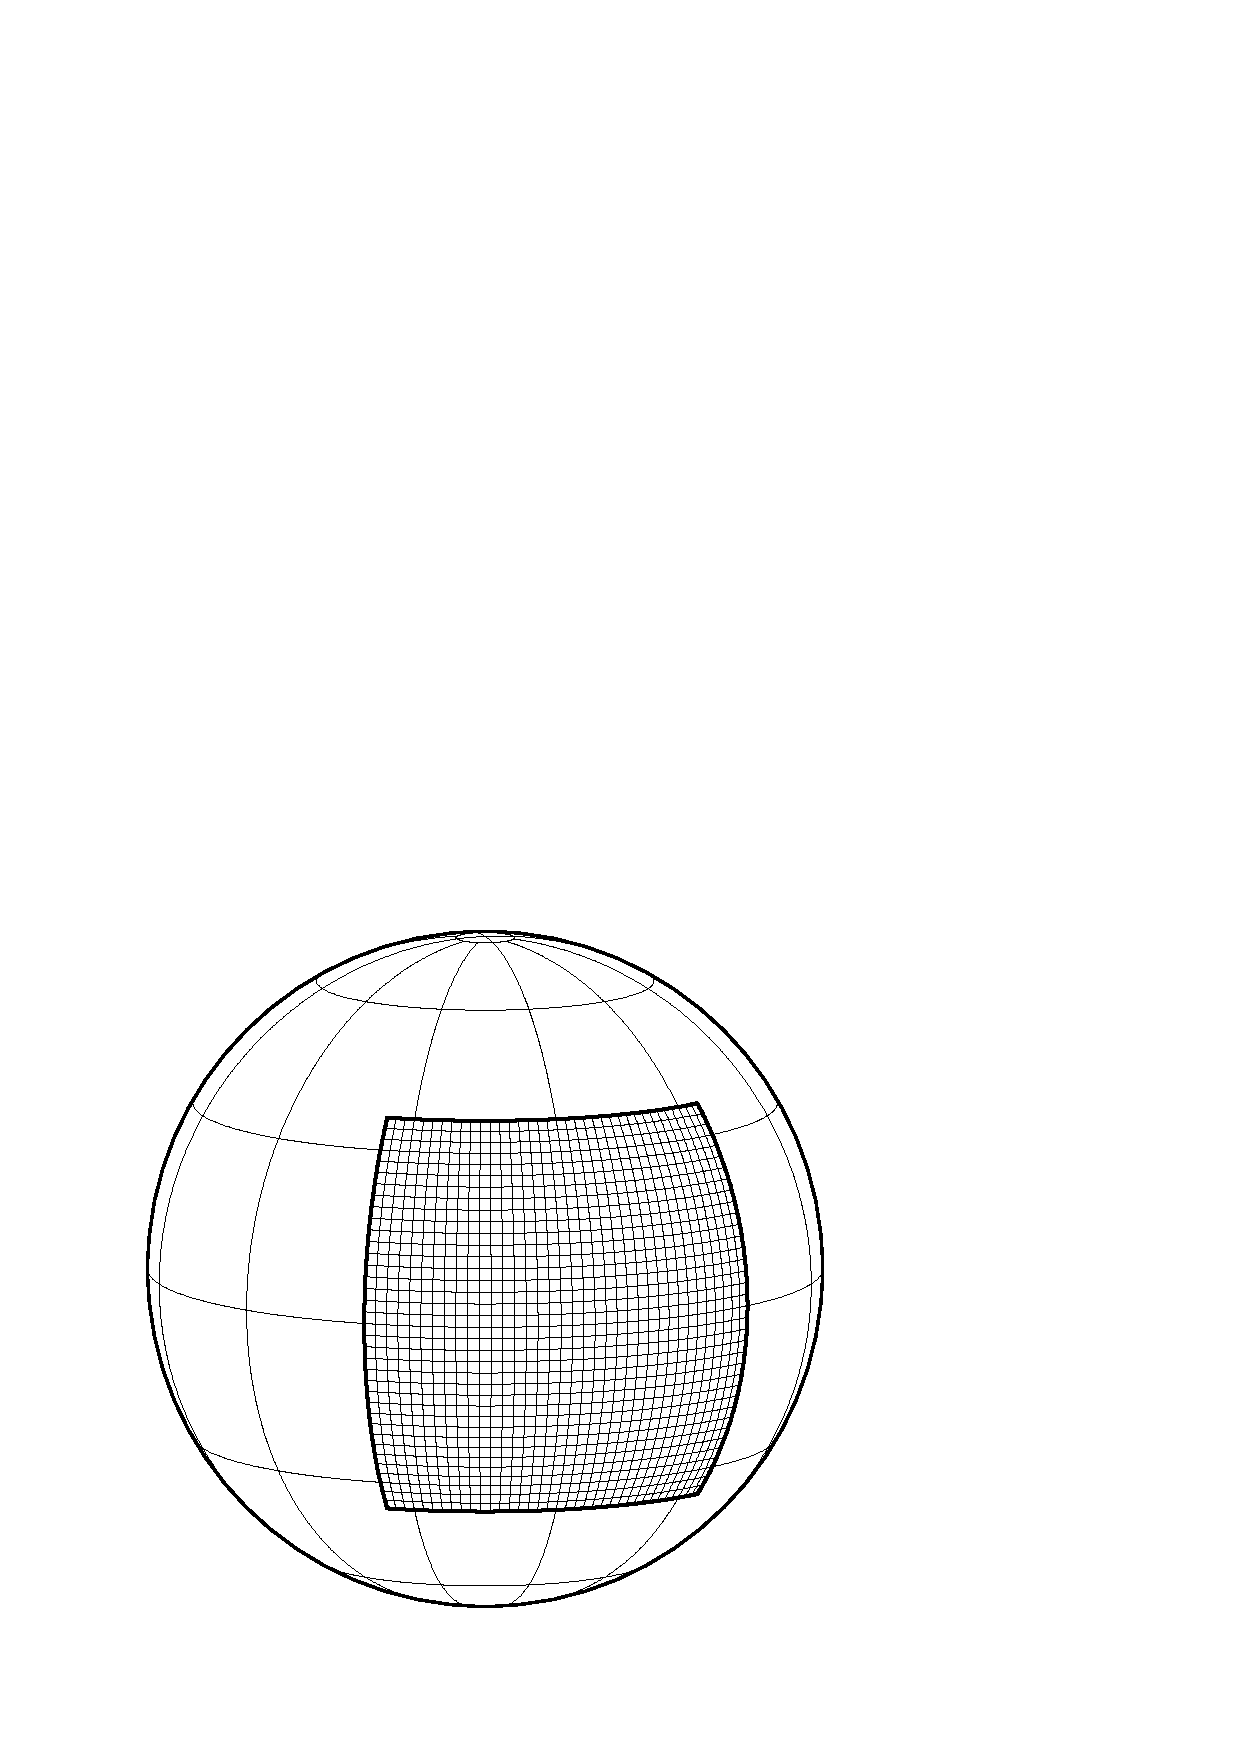
\includegraphics[angle=0,scale=0.5]{Figures/Apx_Test/LLfig_lowres.png}
\includegraphics[angle=0,scale=0.25]{Figures/Apx_Test/TC1_basemap.png}
\parbox{15cm}{\caption{\label{FigTest_ConvTC1_grid}
Grid and example advection for Test Case 1.1
}}
\end{figure}
The test is initially conducted on a Cartesian grid, then repeated on a longitude/latitide
grid. The windfield is homogeneous and constant for the Cartesian case, but
heterogeneous in the longitude/latitude case, corresponding to rigid-body rotation
on a sphere.

\begin{figure}[htbp]\vspace*{0cm}\hspace*{0cm}
\includegraphics[angle=0,scale=0.3]{Figures/Apx_Test/TC1_LL_Sub5.png}
\parbox{15cm}{\caption{\label{FigTest_ConvTC15_grid}
Convergence plot for TC1.5. The top row is for the mid-point; bottom
row is for the boundary. Left column is the $L_1$ error; right column
is the mass concervation error.
}}
\end{figure}

\subsection{Test case 2: Vertical advection of smooth source}
Test case 2 isolates the vertical advection routines and uses the same set-up as in
Test case 1. There are four sub-cases
(SC1:$v_z+$,$V_f=0$; SC2:$v_z-$,$v_f=0$; SC3:$v_z=0$,$v_f+$; SC4:$v_z=0$,$v_f-$).
These tests are only for a Cartesian grid.
\begin{figure}[htbp]\vspace*{0cm}\hspace*{0cm}
\includegraphics[angle=0,scale=0.3]{Figures/Apx_Test/TC1_LL_Sub5.png}
\parbox{15cm}{\caption{\label{FigTest_ConvTC21_grid}
Convergence plot for TC2.1.
}}
\end{figure}

\subsection{Test case 3: Horizontal rotational advection of 2-D cone and box}
This test case examines the effect of rigid-body rotation of a concentration profile
through one revolution.  The concentration profile is given below for a Cartesian grid
and consists of a cone centered at $x=-0.45$, $y=0$ and a box located at
$0.1<x<0.6$, $-0.25<y<0.25$.
%  \begin{linenomath*}
\begin{eqnarray}\label{EqTC3sol}
q_0 &=& \left\{ \begin{array} {l@{\quad \quad}l}
1         &:  \mathrm{if}\,\,\, 0.1 < x < 0.6 \,\,\mathrm{and}\\
          &  \,\,\, -0.25 < y < 0.25 \\
1-r/0.35  &:  \mathrm{if}\,\,\, r < 0.35 \\
0         &: \mathrm{Otherwise}
\end{array}
\right.
\end{eqnarray}
%  \end{linenomath*}
where $r \equiv \sqrt{\left( x+0.45\right)^2+y^2}$.
The wind field is given by
%  \begin{linenomath*}
\begin{eqnarray}
u(x,y)=2y & & v(x,y)=-2x \label{EqTC3Wind}
\end{eqnarray}
%  \end{linenomath*}

\begin{figure}[htbp]\vspace*{0cm}\hspace*{0cm}
\includegraphics[angle=0,scale=0.3]{Figures/Apx_Test/TC3_LL_compare.png}
\includegraphics[angle=0,scale=0.3]{Figures/Apx_Test/TC3_LL_Solution_Error_L1.png}
\parbox{15cm}{\caption{\label{FigTest_ConvTC3}
Solution plot for TC3 and convergence behaviour.
}}
\end{figure}
Figure \ref{EqTC3sol} shows that the DCU implementation of advecting in x, then advecting
in y (switching the order with each time step), introduces a splitting error and reduces
the order of accuracy to 1rst order.

\subsection{Test case 4: 1-D diffusion}
This test case checks the implementation of the diffusion routines along the three
coordinate axes. The model consists of diffusion with a discontinuous initial
concentration and with a diffusivity contrast at the origin. There are 6 sub-cases for
this test for diffusion along x, y, and z with the explicit solver, then repeating
x, y, and z with the Crank-Nicolson solver.

\begin{figure}[htbp]\vspace*{0cm}\hspace*{0cm}
\includegraphics[angle=0,scale=0.3]{Figures/Apx_Test/TC4_XY_Solution_Sub1.png}
\includegraphics[angle=0,scale=0.3]{Figures/Apx_Test/TC4_XY.png}
\parbox{15cm}{\caption{\label{FigTest_ConvTC4}
Solution plot for TC4 and convergence behaviour.
}}
\end{figure}
The current implementation of diffusion is 2nd order for homogeneous diffusivities, but
is reduced to 1rst order for heterogeneous diffusivities.


\subsection{Test case 5: Reversible horizontal shearing}
To evaluate the ability of these numerical schemes to track advection in highly
deforming wind fields, a test was run using a transient, rotational wind field
where the rotational velocity about the pole
($\phi_0=0^{\circ}$, $\lambda_0=0^{\circ}$) is given by (shown in figure b)
%  \begin{linenomath*}
\begin{equation}\label{EqTC5Wind}
\omega(\phi,\lambda) = -0.5\sin(d\pi/18) \cos(\pi t/4)
\end{equation}
%  \end{linenomath*}
where $d$ is the angular distance (in degrees) of $\phi$, $\lambda$ from $\phi_0$, $\lambda_0$.
The initial concentration distribution (shown in figure a) is given by
%  \begin{linenomath*}
\begin{equation}\label{EqTC5Source1}
q(\lambda,\phi,z,t=0)=0.5 (1.0+\cos(\pi r))
\end{equation}
%  \end{linenomath*}
where $r$ is given by:
%  \begin{linenomath*}
\begin{eqnarray}
r &=& \sqrt{(\phi+16.0)^2 + \lambda^2/16} \label{EqTC5Source2} \\
r &=& \mathrm{min(}1.0,r) \label{EqTC5Source3}
\end{eqnarray}
%  \end{linenomath*}
\begin{figure}[htbp]\vspace*{0cm}\hspace*{0cm}
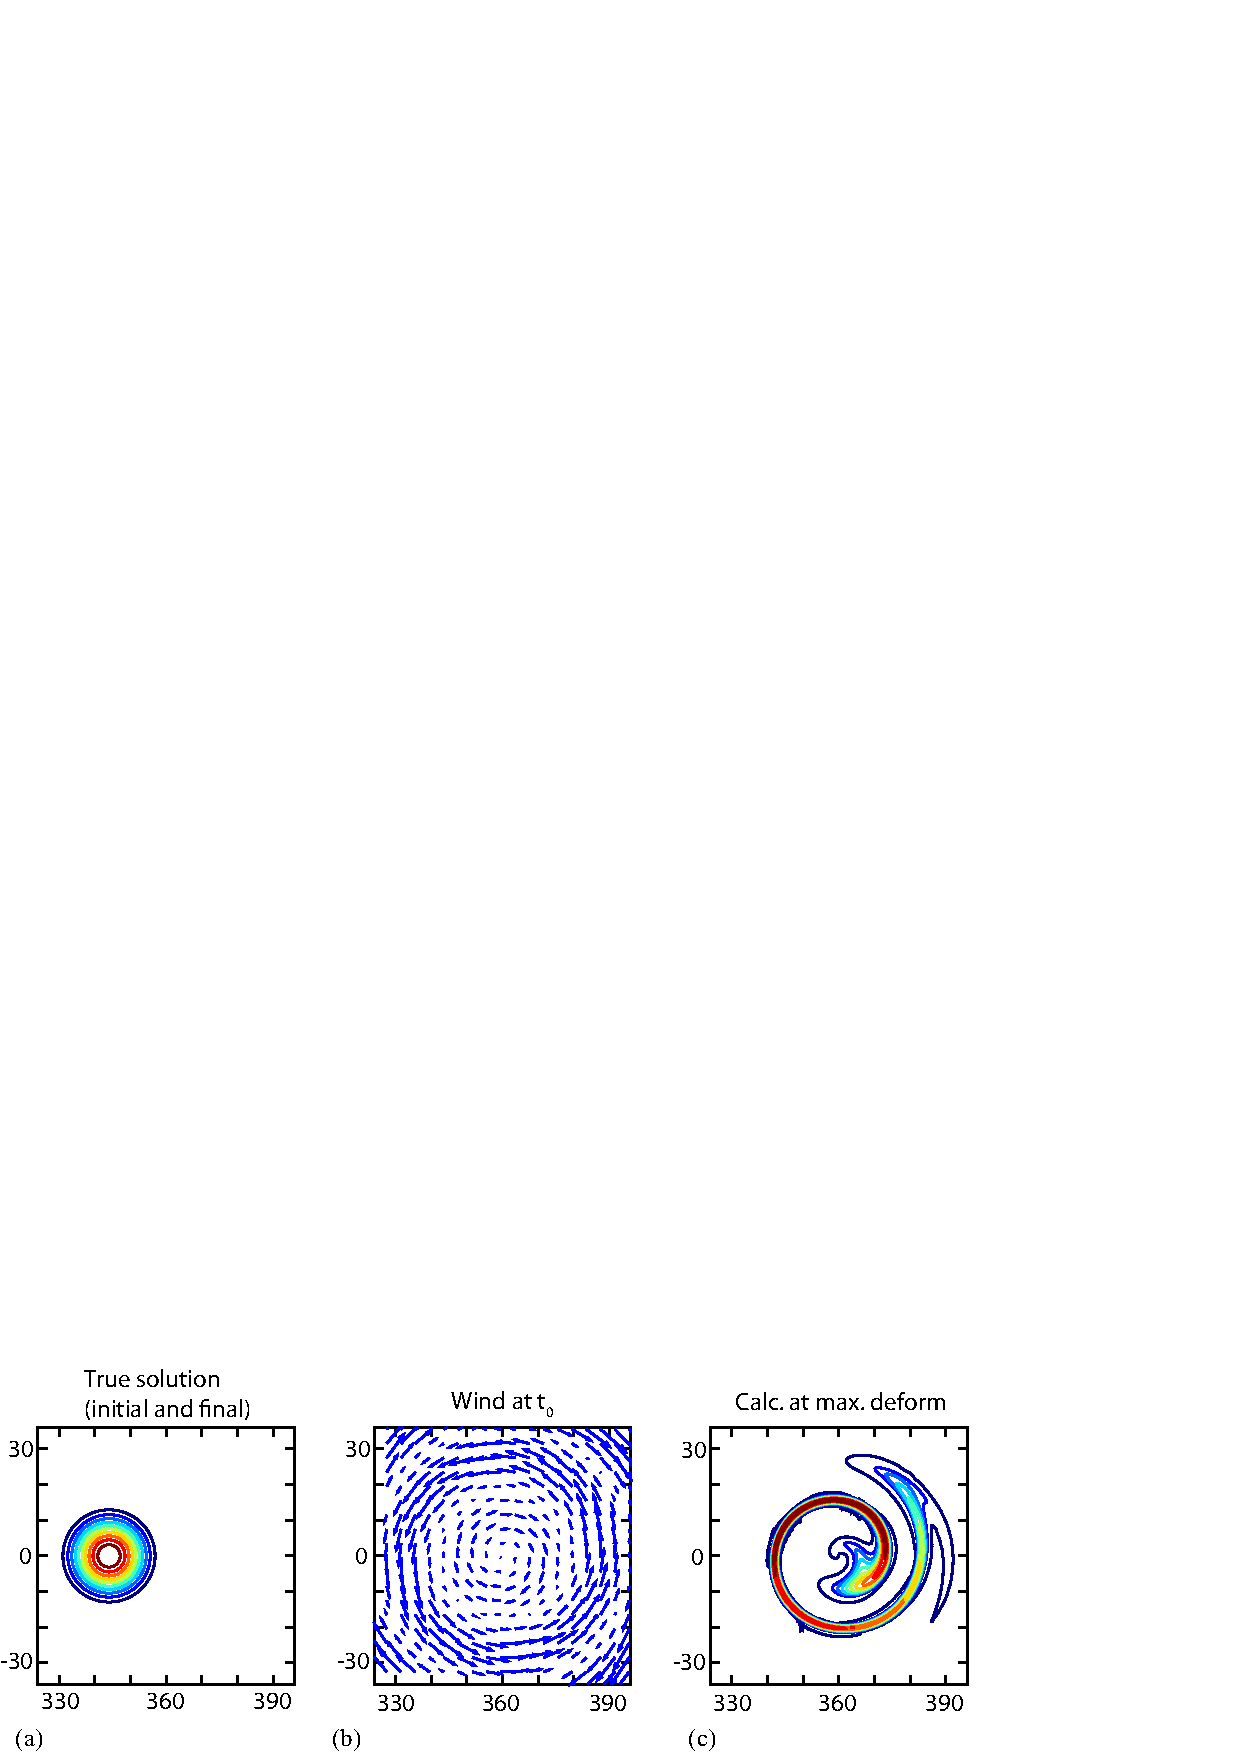
\includegraphics[angle=0,scale=1.0]{Figures/Apx_Test/TC5_Def_Sol.png}
\parbox{15cm}{\caption{\label{FigTest_ConvTC5def}
Initial/final solution for TC5 along with peak deformation.
}}
\end{figure}

The initial concentration distribution is deformed into a long strand at $t=2$ (figure c),
then the deformation reverses back to the initial configuration.  A similar test in
Cartesian coordinates %\citep[Sec. 5.7.4]{Durran1999}
was also conducted.  Versions of the
test cases for both Cartesian and spherical coordinates are shown.

Figure \ref{FigTest_ConvTC5def} shows the behavior of the various numerical
methods for this test problem at $t=4$
when the deformation should return to zero.  Each plot of figure should be compared with
figure a.  Since diffusion is not calculated in this test problem, any distortion of the
final profile is a result of numerical diffusion.  The CTU method without the use of a
limiter recovers the initial profile with the greatest fidelity.  However it is possible
in this case, since the use of limiters is non-linear, that errors in the advection in
the clock-wise rotation are simply reversed in the counter-clock-wise phase of the oscillation.

\begin{figure}[htbp]\vspace*{0cm}\hspace*{0cm}
\includegraphics[angle=0,scale=0.3]{Figures/Apx_Test/TC5_LL_compare.png}
\includegraphics[angle=0,scale=0.3]{Figures/Apx_Test/TC5_LL_Solution_Error_L1.png}
\parbox{15cm}{\caption{\label{FigTest_ConvTC5}
Solution plot for TC5 and convergence behaviour.
}}
\end{figure}

\clearpage
\subsection{Test case 6: Method of manufactured solutions}
In addition to the two test cases shown above (rotational advection and reversible
rotational shear) simple 1-dimensional advection and 1-dimensional diffusion tests
were conducted along the coordinate axis to verify convergence properties.  Simple
tests such as these are useful for identifying obvious bugs in the code; however,
they do not fully test all aspects of the algorithm.  In general, analytic solutions
are not available for the advection-diffusion-sedimentation equation in a non-trivial
wind field with realistic pressure and temperature profiles (See \cite{Stockie2011} for
solutions in simplified atmospheric conditions.).  However, the Method of Manufactured
Solutions (MMS) %\citep{Roache2009,Salari2000}
provides some guidance on how to generate
analytic solutions for non-trivial atmospheric conditions which will invoke all
components of the algorithm, all terms of the governing equation and boundary conditions.
This will allow us to confirm the order of accuracy of the complete algorithm.

If a domain is specified and atmospheric and boundary conditions prescribed, then a
``source" (a transient spatial distribution of tephra characterizing the eruption)
results in a ``solution" (a transient spatial distribution of airborne and deposited
tephra) through the governing equation.  In Eq. \ref{EqGovEqVect}, the source is $S$
and the solution is $q$.  In general, we do not know the solution {\it a priori} that
is the result of the source term and boundary conditions.  The idea behind the Method
of Manufactured Solutions is to find a compatible set of functions for the source and
the solution by specifying $q$ and solving for $S$.

To employ the MMS method, we first choose a model geometry (domain and topography) and
define the physical state ($p$, $T$, $u$, $v$, $w$, $\mathbf{K}$).  Next, we simply
choose a non-trivial solution, $q$, ideally one with a 3-dimensional, transient structure
that is easily differentiable.  This artificial solution need not be physically realistic
since our goal is to evaluate the performance of the algorithm, not model a particular
physical process.  This solution can be inserted into the governing equation
(Eq. \ref{EqGovEqVect}) and evaluated to generate a non-trivial, three-dimensional, transient
source term, $S$.  Note that this source term will not resemble the vertical distribution
described in section \ref{SubSecDepo}, but instead will be a transient three-dimensional
function.  Initial conditions are generated by simply evaluating the chosen solution at
$t=t_0$.  Boundary conditions can be determined by evaluating $q$ along the boundary.
Applying the algorithm with these initial and boundary conditions, along with the source
term, will generate a numerical solution that can be compared with the solution that was
initially chosen.  Grid convergence studies of this test case will quantify the order of
accuracy of the full algorithm.

We use the following domain for the MMS test.
$-100<x<100\, \mathrm{km}$, $-100<y<100\, \mathrm{km}$, $0<z<20 \, \mathrm{km}$.
We use a standard atmosphere for the pressure and temperature profiles given by
%\citet[chap. 1]{Wallace1977}
:  $P = P_0 \exp (-z/\delta)$ and $T = T_0 + \theta z$.
For the wind velocity structure, we adopt a horizontal model to mimic wind shear with small
vertical perturbations:
$u = U_0$, $v = V_0/2\left( 1 + \tanh ( z-Z_0)\right)$,
$w=-W_0 \cos(\pi x/\lambda_{xy})\cos(\pi y/\lambda_{xy})$.
The diffusivity is set to a constant.
The fall model is set via the equations of section \ref{SubSecDepo} using the ideal gas
law and Sutherland's Law to calculate $\rho_a$ and $\eta_a$.

The solution we choose is given below.
%  \begin{linenomath*}
\begin{equation} \label{EqMMSSolution}
q = Q_0 \, \mathrm{sech} \left( \frac{x}{\lambda_{xy}}\right) \mathrm{sech} \left( \frac{y}{\lambda_{xy}}\right)
\mathrm{sech} \left( \frac{z}{\zeta}\right)
\end{equation}
%  \end{linenomath*}
where $\zeta=W_0 t + \zeta_0$.
To calculate the source term, $S$, we need to calculate the first partial derivatives of $q$
with respect to $t$, and both first and second partial derivatives with respect to the
spatial coordinates.
%  \begin{linenomath*}
\begin{eqnarray}
\frac{\partial q}{\partial t} &=& q\left[ z \frac{W_0}{\zeta^2} \mathrm{tanh}(z/\zeta)\right] \label{EqMMSQt} \\
\frac{\partial q}{\partial x} &=& q\left[ -\frac{\tanh (x/\lambda_{xy})}{\lambda_{xy}} \right] \label{EqMMSQx} \\
\frac{\partial^2 q}{\partial x^2} &=& q\left[ \frac{\tanh^2 (x/\lambda_{xy})}{\lambda^2_{xy}} - \frac{\mathrm{sech}^2 (x/\lambda_{xy})}{\lambda^2_{xy}}\right]  \label{EqMMSQxx} \\
%\frac{\partial q}{\partial y} &=& q\left[ -\frac{\tanh (y/\lambda_{xy})}{\lambda_{xy}} \right] \\ \label{EqMMSQy}
%\frac{\partial^2 q}{\partial y^2} &=& q\left[ \frac{\tanh^2 (y/\lambda_{xy})}{\lambda^2_{xy}} - \frac{\mathrm{sech}^2 (y/\lambda_{xy})}{\lambda^2_{xy}}\right] \\ \label{EqMMSQyy}
\frac{\partial q}{\partial z} &=& q \left[ - \frac{\mathrm{tanh}(z/\zeta)}{\zeta}\right]\\ \label{EqMMSQz}
\frac{\partial^2 q}{\partial z^2} &=& q \left[ \frac{1}{\zeta^2}\left( \mathrm{tanh}^2(z/\zeta) - \mathrm{sech}^2(z/\zeta)\right)\right] \label{EqMMSQzz}
\end{eqnarray}
%  \end{linenomath*}
The equations for first and second derivatives in $y$ are of the same form as
Eq.s \ref{EqMMSQx} and \ref{EqMMSQxx}.
The choice of Eq. \ref{EqMMSSolution} is not unique, but is guided by the simple form of
the derivatives in Eq.s \ref{EqMMSQt}--\ref{EqMMSQzz}.  An arbitrarily complex form of
$q$ can be chosen, as determining $S$ is straight-forward once the derivatives are
calculated; although it may be more cumbersome to implement. Assembling these terms into
the governing equation (Eq. \ref{EqGovEqVect}) leads to a simple expression for the source
term, $S$, which is a continuous function of space and time.  By selecting individual
constants (i.e. $U_0$, $V_0$, $W_0$, $Z_0$, $\zeta_0$) we can selectively activate or
deactivate branches of the algorithm.  If all are activated, we have an analytic solution
against which we can compare the full advection-diffusion-sedimentation equation.  This is
particularly important for calculating splitting errors due to the decomposition of the
governing equation via the method of fractional steps. The constants used in the testcase
are given in Table \ref{TabMMSConsts}.

$L_1$-norm convergence results are shown in figure \ref{FigMMSConverge}.  The full
simulation using the semi-Lagrangian scheme for the horizontal advection produce results
that converge with an order accuracy of 1.5.
Without the use of limiters, the DCU and CTU schemes converge with second-order accuracy.
With minmod, superbee and MC limiters, the accuracy of the calculations with DCU and CTU
for horizontal advection reduces to approximately order 1.8.  The fact that these
convergence rates are nearly second-order suggests that splitting errors are minimal.
Although the use of limiters in this particular case reduces the order of convergence
slightly, they significantly improve the resolution of sharp boundaries.

\begin{figure}[htbp]\vspace*{0cm}\hspace*{0cm}
\includegraphics[angle=0,scale=0.4]{Figures/Apx_Test/TC5_XY_Solution_Error_L1.png}
\parbox{15cm}{\caption{\label{FigTest_ConvTC6def}
Convergence behaviour for Test Case 6.
}}
\end{figure}


\clearpage
\section{Validation Testing}
\subsection{Spurr (Deposit): August 19, 1992}
\begin{figure}[htbp]
\includegraphics[angle=0,scale=0.6]{Figures/TestCase_Results/ValidTest/Spurr_Deposit.pdf}
\parbox{15cm}{\caption{\label{FigTestValSpurr} Deposit}}
\end{figure}

\clearpage
\subsection{Mt. St. Helens (Deposit with Aggregates): May 18, 1980}
\begin{figure}[htbp]
\includegraphics[angle=0,scale=0.6]{Figures/TestCase_Results/ValidTest/MSH_Deposit.pdf}
\parbox{15cm}{\caption{\label{FigTestValMSH} Deposit}}
\end{figure}

\clearpage
\subsection{Kasatochi (Ash cloud load): August 8, 2008}
\begin{figure}[htbp]
\includegraphics[angle=0,scale=0.3]{Figures/TestCase_Results/ValidTest/Kasatochi_CloudLoad_0.pdf}
\includegraphics[angle=0,scale=0.3]{Figures/TestCase_Results/ValidTest/Kasatochi_CloudLoad_1.pdf}
\includegraphics[angle=0,scale=0.3]{Figures/TestCase_Results/ValidTest/Kasatochi_CloudLoad_2.pdf}
\includegraphics[angle=0,scale=0.3]{Figures/TestCase_Results/ValidTest/Kasatochi_CloudLoad_3.pdf}
\includegraphics[angle=0,scale=0.3]{Figures/TestCase_Results/ValidTest/Kasatochi_CloudLoad_4.pdf}
\includegraphics[angle=0,scale=0.3]{Figures/TestCase_Results/ValidTest/Kasatochi_CloudLoad_5.pdf}
\includegraphics[angle=0,scale=0.3]{Figures/TestCase_Results/ValidTest/Kasatochi_CloudLoad_6.pdf}
\includegraphics[angle=0,scale=0.3]{Figures/TestCase_Results/ValidTest/Kasatochi_CloudLoad_7.pdf}
\parbox{15cm}{\caption{\label{FigTestValKasatochi} Cloud load}}
\end{figure}

\clearpage
\subsection{Mazama (Deposit from Umbrella Source)}
\begin{figure}[htbp]
\includegraphics[angle=0,scale=0.6]{Figures/TestCase_Results/ValidTest/Mazama_UmbrellaDeposit.pdf}
\parbox{15cm}{\caption{\label{FigTestValMazama} Deposit}}
\end{figure}

\clearpage
\subsection{Kelud (Ash Cloud from Umbrella Source), Feb. 13, 2014}
\begin{figure}[htbp]
\includegraphics[angle=0,scale=0.3]{Figures/TestCase_Results/ValidTest/Kelud_CloudOutline_0.pdf}
\includegraphics[angle=0,scale=0.3]{Figures/TestCase_Results/ValidTest/Kelud_CloudOutline_1.pdf}
\includegraphics[angle=0,scale=0.3]{Figures/TestCase_Results/ValidTest/Kelud_CloudOutline_2.pdf}
\includegraphics[angle=0,scale=0.3]{Figures/TestCase_Results/ValidTest/Kelud_CloudOutline_3.pdf}
\includegraphics[angle=0,scale=0.3]{Figures/TestCase_Results/ValidTest/Kelud_CloudOutline_4.pdf}
\includegraphics[angle=0,scale=0.3]{Figures/TestCase_Results/ValidTest/Kelud_CloudOutline_5.pdf}
\includegraphics[angle=0,scale=0.3]{Figures/TestCase_Results/ValidTest/Kelud_CloudOutline_6.pdf}
\includegraphics[angle=0,scale=0.3]{Figures/TestCase_Results/ValidTest/Kelud_CloudOutline_7.pdf}
\parbox{15cm}{\caption{\label{FigTestValKelud} Umbrella Cloud Spreading rate}}
\end{figure}

%\subsection{}

